\documentclass[a4paper]{article} 
\usepackage[francais]{babel}
\usepackage[utf8]{inputenc} % Required for including letters with accents
\usepackage[T1]{fontenc} % Use 8-bit encoding that has 256 glyphs
\usepackage{pythontex}
\usepackage{amsthm}
\usepackage{amsmath}
\usepackage{amssymb}
\usepackage{mathrsfs}
\usepackage{graphicx}
\usepackage{geometry}
\usepackage{stmaryrd}
\usepackage{tikz}
\usetikzlibrary{shapes}
\usetikzlibrary{patterns}
\usepackage[cache=false]{minted}
 \definecolor{darkWhite}{rgb}{0.94,0.94,0.94}
 \usepackage[cache=false]{minted}
\definecolor{LightGray}{gray}{0.9}
\definecolor{monOrange}{rgb}{0.97,0.35,0.04}
\def \de {{\rm d}}
\usepackage{color}
\usepackage{xcolor}
\newcommand{\mybox}[1]{\fbox{$\displaystyle#1$}}
\newcommand{\myredbox}[1]{\fcolorbox{blue}{white}{$\displaystyle#1$}}
\newcommand{\mybluebox}[1]{\fcolorbox{blue}{white}{$\displaystyle#1$}}
\newcommand{\mygreenbox}[1]{\fcolorbox{green}{white}{$\displaystyle#1$}}
\newcommand{\mydoublebox}[1]{\fbox{\fbox{$\displaystyle#1$}}}
\newcommand{\myreddoublebox}[1]{\fcolorbox{red}{white}{\fcolorbox{red}{white}{$\displaystyle#1$}}}

\usepackage{geometry}
 \geometry{
 a4paper,
 total={210mm,297mm},
 left=20mm,
 right=20mm,
 top=20mm,
 bottom=20mm,
 }
%%%%%%%%%%%%%%%%%%
\usepackage{tikz}
\usetikzlibrary{patterns}
 
\newcommand*{\Rayon}{0.15}
\newcommand*{\tailleTriangle}{0.5}
\newcommand*{\largeurSol}{1}
\newcommand*{\hauteurSol}{0.4}
\pgfmathsetmacro{\basTriangle}{sin(60)*\tailleTriangle}
\newcommand*{\nbFlechesCont}{10}
\newcommand*{\rayonCouple}{0.1}
\newcommand*{\angleCouple}{110}
 
 
\tikzset{
	sol/.pic ={
		\draw[thick](-\largeurSol/2,0)--(\largeurSol/2,0);
		\fill[fill,pattern=north east lines] (-\largeurSol/2,0) rectangle++ (\largeurSol,-\hauteurSol);
	},
	mur/.pic ={
		\draw[thick](0,-\largeurSol/2)--(0,\largeurSol/2);
		\fill[fill,pattern=north east lines] (0,-\largeurSol/2) rectangle++ (\hauteurSol,\largeurSol);
	},	
	triangle/.pic ={
		\draw(0,0)--++(-60:\tailleTriangle)--++(-\tailleTriangle,0)--cycle;
		\node[anchor=south]{ \tikzpictext};
	},
	pivot/.pic ={
		\pic{triangle};
		\pic at (0,-\basTriangle){sol};
	},
	ponctuelle/.pic ={
		\pic{triangle};
		\draw(-\Rayon,-\basTriangle-\Rayon) circle(\Rayon);
		\draw(\Rayon,-\basTriangle-\Rayon) circle(\Rayon);
		\pic at(0,-\basTriangle-2*\Rayon){sol};
	},
	encastrd/.pic ={
		\pic{mur};
		\node{ \tikzpictext};		
	},
	encastrg/.pic ={
		\pic[xscale=-1]{mur};
		\node{ \tikzpictext};		
	}	
}
\newcommand{\chargecont}[4][]{% #1 (optionnel) style, #2 point de départ, #3 longueur, #4 nom de la charge
	\pgfmathsetmacro{\pas}{#3/\nbFlechesCont}
	\foreach \x in {0,\pas,...,#3}{
		\draw[latex-,#1] ([xshift=\x cm]C) --++(0,0.5);
	}
	\draw[#1]([yshift=0.5 cm]#2)--++(#3,0) node[midway,above]{#4};
}
\newcommand{\couple}[3][]{% #1 (optionnel) style, #2 point d'application, #3 nom du couple
	\draw[->,#1] (#2) +(\angleCouple:\rayonCouple) arc(\angleCouple:-\angleCouple:\rayonCouple) node[anchor=north] {$\mathcal{C}$};
}

%%%%%%%%%%%%%%%%%%%
\title{Projet numérique: calcul des structures, Barres et poutres}
\author{Ibrahim ALAME}
\date{21/03/2024}
\begin{document}
\maketitle

La  première partie du projet est consacrée à la formulation d'une barre (ou de treillis) qui permet d'analyser des structures constituées de poutres articulées aux deux extrémités  et qui ne transmettent que des efforts de traction compression aux nœuds d'assemblages. Sur le plan pratique, cela permet d'évaluer rapidement la distribution des efforts dans les structures de type pylônes, ossatures, toitures en treillis métalliques, etc.
La deuxième partie traite des portiques ...

Considérons une barre homogène de module $E$, section constante $A$ et de longueur $L$ soumise à une sollicitation $f(x)$. Les équations du problème sont:
\subsubsection*{Équation d'équilibre}

\begin{center}
 \begin{tikzpicture}[scale=1]
\draw  [very thin, gray] [->]  (-2,0) -- (9.5,0) node[right] {$x$};
\fill[cyan] (3,-0.5) rectangle (4,0.5);
\draw[orange,thick=2] (0,-0.5) rectangle (7,0.5);
\draw[very thick,olive,<-] (2,0) -- (3,0) node[below, midway]{$\scriptstyle -\vec{N}(x)$};
\draw[very thick,olive,->] (4,0) -- (5.2,0) node[below, midway]{$\scriptstyle \vec{N}(x+dx)$};
\draw[cyan,<->] (3,0.7) -- (4,0.7) node[above,midway ]{$\scriptstyle dx$};
\draw[cyan,<->]  (4,0.7)--(4.2,0.7) node[above,midway ]{$\scriptstyle du$};
\draw[cyan,dashed]  (4.2,-0.5)--(4.2,0.5);
\draw[very thick,olive,->] (3.5,0) -- (3.5,-1) node[below]{$\scriptstyle \vec{p}(x)dx$};
\draw[very thick,red,->]  (0,0) --(-1.5,0) node[above]{$\scriptstyle -\vec{f}_1$};
\draw[very thick,red,->]  (7,0) --(8.5,0) node[above]{$\scriptstyle \vec{f}_2$};
%\draw [domain=0:5][line width=1] plot(\x,{.8598e-1*\x*\x*\x-.8104*\x*\x+1.697*\x});
%\draw [domain=0:6] plot(\x,{sin(57.29*\x)});
\end{tikzpicture} 

\end{center}

Nous avons
\[N(x+dx)-N(x)+p(x)\de x=0\, \Longrightarrow \frac{\de N(x)}{\de x}\de x+p(x)\de x=0\, \Longrightarrow \myredbox{\frac{\de N(x)}{\de x}+p(x)=0}\]
Dans la suite du projet, nous allons négliger les forces linéiques $p(x)\simeq 0$.
\subsubsection*{Loi de comportement }
On applique la loi de Hooke: $\sigma = E \varepsilon $ où $E$ est le module de Young, $\sigma$ est la contrainte $\frac{N}{A}$ et $\varepsilon=\varepsilon_1-\color{red}{\varepsilon_2}$ est la déformation élastique: $\varepsilon_1=\frac{\de u}{dx}$ (déformation totale) et $\color{red}{\varepsilon_2=\alpha \Delta T}$ (déformation thermique), où $\alpha$ est le coefficient de dilatation linéaire.
\[ \sigma = E \varepsilon \Longrightarrow\frac{N}{A}=E (\varepsilon_1-\varepsilon_2)\,\Longrightarrow  \myredbox{N=EA\left(\frac{\de u}{dx}{\color{red}{-\alpha \Delta T}}\right)}\]

\subsubsection*{Problème à résoudre}

\[
\left\{
\begin{array}{lcr}
\displaystyle \frac{\de N}{\de x}=0;&0\leq x\leq L &\mbox{ équation d'équilibre } \\
N=EA\displaystyle \left(\frac{\de u}{dx}{\color{red}{-\alpha \Delta T}}\right)& 0\leq x\leq L&\mbox{ loi de comportement } \\
u(0)=u_1 ;u(L)=u_2&&\quad\mbox{ conditions aux limites } \\
N(0)=-f_1 ;N(L)=f_2&&\quad\mbox{ conditions aux limites } 
\end{array}
\right.
\]



L'objectif est d'exprimer les efforts $N(x)$ aux extrémités $x=0$ et $x=L$ en fonctions des déplacements aux extrémités $u_1$ et $u_2$ sous forme matricielle.

L'équation d'équilibre et la loi de comportement donnent:

\[\int_0^LN(x)\mbox{d}x=EA\int_0^L \left(\frac{\de u}{dx}{\color{red}{-\alpha \Delta T}}\right)\mbox{d}x\]
\[L\,N= EA\left[(u_2-u_1){\color{red}{-\alpha \Delta T\; L}}\right]\]

On a donc
\[N_{0}=N_L=\frac{EA}{L}(u_2-u_1){\color{red}{-\alpha EA\,\Delta T }}\]


Les efforts appliqués par la barre sur le nœud 1 et 2 s'écrivent sous forme matricielle:
\[\left(\begin{array}{r} 
-N_{0}\\N_{L}
\end{array}\right)=\frac{EA}{L}\left(\begin{array}{rr} 
1&-1\\-1&1
\end{array}\right) \left(\begin{array}{l} 
u_{1}\\u_{2}
\end{array}\right){\color{red}{-\alpha EA\, \Delta T }\left(\begin{array}{c} 
-1\\1
\end{array}\right)}
\]
D'où
\[\myredbox{\left(\begin{array}{r} 
f_{1}\\f_{2}
\end{array}\right)=\frac{EA}{L}\left(\begin{array}{rr} 
1&-1\\-1&1
\end{array}\right) \left(\begin{array}{l} 
u_{1}\\u_{2}
\end{array}\right){\color{red}{-\alpha  EA\, \Delta T }\left(\begin{array}{c} 
-1\\1
\end{array}\right)}}
\]

\begin{center}
 \begin{tikzpicture}[scale=1]
\draw  [very thin, gray] [->]  (-0.2,0) -- (7,0) node[right] {$x$};
\draw (1.2,0.3) node[above] {$u_1$};
\draw (5.25,0.3) node[above] {$u_2$};
\fill[cyan] (1,-0.1) rectangle (5,0.1);
\draw[red,thick=2] (1.4,-0.1) rectangle (5.5,0.1);
\draw[dotted,<->] (1,0.3) -- (1.4,0.3);
\draw[dotted,<->] (5,0.3) -- (5.5,0.3);
\draw[very thick,olive,<-] (0,0) -- (1.4,0) node[below, midway]{$\vec{f_1}$};
\draw[very thick,olive,->] (5.5,0) -- (6.5,0) node[below, midway]{$\vec{f_2}$};

%\draw [domain=0:5][line width=1] plot(\x,{.8598e-1*\x*\x*\x-.8104*\x*\x+1.697*\x});
%\draw [domain=0:6] plot(\x,{sin(57.29*\x)});
\end{tikzpicture} 

\end{center}

\section{Treillis en dimension 2}
Un treillis est un ensemble de barres ou poutres droites reliées entre elles par des nœuds en  rotules. Les liaisons extérieures sont des rotules et des appuis simples. Les charges sont des forces portées par les rotules, des gradients thermiques et des déplacements d'appui. La force intérieure dans une section droite se réduit à l'effort normal.
Le treillis est plan si :
\begin{itemize}
\item Le plan $\{O; x, y\}$ est un plan de symétrie pour toutes les sections droites.
\item Les forces appliquées sont situées dans le plan $\{O; x, y\}$ . On suppose que les déplacements sont petits.
\end{itemize}
\subsection{Matrice de rigidité élémentaire}
Dans la section précédente, les matrices et vecteurs sont définis dans les repères locaux $(x,y)$. L'opérateur d'assemblage (passage de la matrice élémentaire d'une barre à la matrice globale du système) nécessite la transformation des caractéristiques élémentaires des repères locaux dans un repère global $(X,Y)$.
\begin{center}
 \begin{tikzpicture}[scale=1]
\draw  [very thin, gray] [->]  (-0.2,0) -- (4,0); 
\draw  [very thin, gray] [->] (0,-0.2) -- (0,3);
\draw  [dashed] (1,0) -- (1,.5)--(0,.5);
\draw  [dashed] (3,0) -- (3,2.5)--(0,2.5);
\draw (1,0) node[below] {$X_i$};
\draw (3,0) node[below] {$X_j$};
\draw (-0.2,0.5) node[below] {$Y_i$};
\draw (-0.2,2.5) node[below] {$Y_j$};
\draw [double distance = 3pt] (1,0.5) -- (3,2.5);
\path[fill=black]  (1,.5) circle (1.2mm) [fill=gray];
\path[fill=black]  (3,2.5) circle (1.2mm) [fill=gray];
\coordinate (A) at (2,.5);
\draw[->,red] (A)  arc(0:45:1);
\draw[red] (2,.9) node[right]{$\theta$};
\draw  [dotted] (1,.5) -- (3,.5);
\draw  [very thin, gray] [->]  (0.8,0.3) -- (3.5,3.); 
\draw  [very thin, gray] [->] (1.2,0.3) -- (-1,2.5);
\draw (4,0) node[right] {$X$};
\draw (0,3.2) node[right] {$Y$};
\draw (3.5,3) node[right] {$x$};
\draw (-1,2.8) node[right] {$y$};
%\draw [domain=0:5][line width=1] plot(\x,{.8598e-1*\x*\x*\x-.8104*\x*\x+1.697*\x});
%\draw [domain=0:6] plot(\x,{sin(57.29*\x)});
\end{tikzpicture} 

\end{center}
Une variable nodale d'une poutre s'exprime dans le repère local $(Ox)$, par un vecteur $\left(\begin{array}{l} 
v_{1}\\v_{2}
\end{array}\right)$ et  dans le repère global $(\Omega XY)$, par le vecteur
\[\left(\begin{array}{l} 
\vec{V_{1}}\\\vec{V_{2}}
\end{array}\right) =\left(\begin{array}{l} 
V_{1}^x\\V_{1}^y\\V_{2}^x\\V_{2}^y
\end{array}\right)  \]


\begin{center}
 \begin{tikzpicture}[scale=1]
\draw  [very thin, gray] [->]  (-0.2,0) -- (4.5,0); 
\draw  [very thin, gray] [->] (0,-0.2) -- (0,3.5);
\draw  [dashed] (1,0) -- (1,.5)--(0,.5);
\draw  [dashed] (3,0) -- (3,2.5)--(0,2.5);
\draw [blue,->,line width=1.6pt] (1,0)--(1.5,0) node[below left] {$V_{1}^x$};
\draw  [blue,dashed] (1.5,0) -- (1.5,1);
\draw  [blue,dashed] (1.5,1) -- (0,1);
%\draw (3,0) node[below] {$X_r$};
\draw [blue,->,line width=1.6pt] (0,0.5)--(0,1) node[left] {$V_{1}^y$};
%\draw (-0.2,2.8) node[below] {$Y_r$};
\draw [double distance = 3pt] (1,0.5) -- (3,2.5);
\path[fill=gray]  (1,.5) circle (1.2mm); %[fill=gray] node[above left]{$q$};
\draw  [blue,->,line width=1.6pt] (1,.5) -- (1.5,1) node[above left]{$v_1$};
\path[fill=gray]  (3,2.5) circle (1.2mm);% [fill=gray] node[above left]{$r$};
\draw  [red,->,line width=1.6pt] (3,2.5) -- (3.5,3) node[above left]{$v_2$};
\draw  [red,->,line width=1.6pt] (3,0) -- (3.5,0) node[below left]{$V_{2}^x$};
\draw  [red,->,line width=1.6pt] (0,2.5) -- (0,3) node[left]{$V_{2}^y$};
\draw  [red,dashed] (3,0) -- (3,2.5);
\draw  [red,dashed] (3.5,0) -- (3.5,3);
\draw  [red,dashed] (0,3) -- (3.5,3);
\coordinate (A) at (2,.5);
\draw[->,red] (A)  arc(0:45:1);
\draw[red] (2,.9) node[right]{$\theta$};
\draw  [dotted] (1,.5) -- (4,.5);
\draw  [very thin, gray] [->]  (0.8,0.3) -- (4,3.5); 
%\draw  [very thin, gray] [->] (1.2,0.3) -- (-1,2.5);
\draw (4.5,0) node[right] {$X$};
\draw (0,3.7) node[right] {$Y$};
\draw (4,3.5) node[right] {$x$};
%\draw (-1,2.8) node[right] {$y$};
%\draw [domain=0:5][line width=1] plot(\x,{.8598e-1*\x*\x*\x-.8104*\x*\x+1.697*\x});
%\draw [domain=0:6] plot(\x,{sin(57.29*\x)});
\end{tikzpicture} 
\end{center}
\begin{enumerate}
\item Justifier rapidement les deux formules suivantes de passage entre les deux repères local $(x,y)$ et global $(X,Y)$:
\[\left(\begin{array}{l} 
v_{1}\\v_{2}
\end{array}\right) = \left(\begin{array}{cccc} 
\cos\theta &\sin\theta&0&0\\
0&0&\cos\theta &\sin\theta
\end{array}\right) \left(\begin{array}{l} 
V_{1}^x\\V_{2}^x\\V_{1}^y\\V_{2}^y
\end{array}\right)  \quad \mbox{et}\quad\left(\begin{array}{l} 
V_{1}^x\\V_{2}^x\\V_{1}^y\\V_{2}^y
\end{array}\right)   = \left(\begin{array}{cc} 
\cos\theta &0\\
\sin\theta& 0\\
0&\cos\theta \\
0 &\sin\theta
\end{array}\right)  \left(\begin{array}{l} 
v_{1}\\v_{2}
\end{array}\right)  \]
\item  En déduire le système élémentaire d'une barre faisant un angle $\theta$ avec $(OX)$:
\[\left(\begin{array}{l} 
F_{2q}\\F_{2q+1}\\F_{2r}\\F_{2r+1}
\end{array}\right)   = \frac{EA}{L}\left(\begin{array}{rrrr} 
c^2&cs&-c^2&-cs\\
cs&s^2&-cs&-s^2\\
-c^2&-cs&c^2&cs\\
-cs&-s^2&cs&s^2
\end{array}\right)\left(\begin{array}{l} 
U_{2q}\\U_{2q+1}\\U_{2r}\\U_{2r+1}
\end{array}\right)  \]
où  $c=\cos\theta$ et $s=\sin\theta$. $\theta$ est défini par
\[\cos \theta = \frac{X_2-X_1}{L}\mbox{ et }\sin \theta = \frac{Y_2-Y_1}{L},\quad L=\sqrt{(X_2-X_1)^2+(Y_2-Y_1)^2} \]
\end{enumerate}






\subsection{Exemple 1: Treillis soumis à une force nodale}
\subsubsection{Énoncé }
Le treillis plan à nœuds  articulés représenté sur la figure 4 est composé de trois poutres de même nature et de même section droite.
Soient $E$ le module de Young du matériau et $A$ l'aire des sections droites.
\begin{itemize}
\item Le noeud 1 est articulé et le nœud 3 repose sur un appui simple dont la normale est horizontale.
\item Le noeud 2 porte une charge de composantes (0, P ).
\end{itemize}
 Application numérique : on donne :
$A=100\mbox{mm}^2$ , $L=0.2 m$ , $E=200000$MPa , $P =-10000$N.
\begin{center}
 \begin{tikzpicture}[scale=1]
\draw  [very thin, gray] [->]  (-2.5,0) -- (4,0); 
\draw  [very thin, gray] [->] (0,-6) -- (0,2.5);
\draw [double distance = 3pt] (0,0) -- (3,0) -- (0,-3*1.732) -- (0,0);
\path[fill=black]  (0,0) circle (2mm) [fill=gray];
\path[fill=black]  (3,0) circle (2mm) [fill=gray];
\path[fill=black]  (0,-3*1.732) circle (2mm) [fill=gray];
\draw [red,->,very thick] (3,0)-- (3,-2) node[right,midway]{$\vec{f_3}=\vec{P}$};
\draw [blue,->,very thick] (0,0)-- (-1.5,0) node[below,midway]{$\vec{f_0}$};
\draw [blue,->,very thick] (0,0)-- (0,1.5) node[right,midway]{$\vec{f_1}$};
\draw [blue,->,very thick] (0,-3*1.732)-- (1.2,-3*1.732) node[below,midway]{$\vec{f_4}$};
\draw (4,0) node[right] {$X$};
\draw (0,2.3) node[right] {$Y$};
%\draw [domain=0:5][line width=1] plot(\x,{.8598e-1*\x*\x*\x-.8104*\x*\x+1.697*\x});
%\draw [domain=0:6] plot(\x,{sin(57.29*\x)});
\end{tikzpicture} 

\end{center}

Les caractéristique géométriques du système se résume en:\\

\begin{tabular}{|l|c|r|}
  \hline
  nœud & $x$  & $y$ \\
  \hline
  0 & 0 & 0 \\
  1& $L$& 0 \\
  2& 0 & $-\sqrt 3 L$ \\
  \hline
\end{tabular} $\hspace{1cm}$  \begin{tabular}{|l|c|r|c|c|}
  \hline
  poutre & $\ell$  & $\theta$ & $C=\cos\theta$ & $S=\sin\theta$\\
  \hline
  (0,1) & $L$ & 0 & 1 & 0 \\
  (1,2)& $2L$& $-\frac{2\pi}{3}$&$-1/2$&$-\sqrt 3/2 $\\
  (2,0)& $\sqrt 3L$ &$\frac{\pi}{2}$ &0 &1 \\
  \hline
\end{tabular}
\\
\\
Écrivons l'équation d'équilibre pour chaque barre:
\[ \left(\begin{array}{r}f_0\\ f_1\\f_2\\f_3 \end{array}\right) 
 =\frac{EA}{L}\left(\begin{array}{rrrr} 
1&0&-1&0\\
0&0&0&0\\
-1&0&1&0\\
0&0&0&0
\end{array}\right)\times
\left(\begin{array}{r} \delta_0\\\delta_1\\\delta_2\\\delta_3 \end{array}\right) 
; \qquad
\left(\begin{array}{r}f_2\\ f_3\\f_4\\f_5 \end{array}\right) 
=\frac{EA}{8L}\left(\begin{array}{rrrr} 
1&\sqrt 3&-1&-\sqrt 3\\
\sqrt 3&3&-\sqrt 3&-3\\
-1&-\sqrt 3&1&\sqrt 3\\
-\sqrt 3&-3&\sqrt 3&3\\
\end{array}\right)\times
\left(\begin{array}{r} \delta_2\\ \delta_3\\\delta_4\\\delta_5 \end{array}\right) 
\]

\[\left(\begin{array}{r}f_4\\ f_5\\f_0\\f_1 \end{array}\right) 
=\frac{EA}{\sqrt 3L}\left(\begin{array}{rrrr} 
0&0&0&0\\
0&1&0&-1\\
0&0&0&0\\
0&-1&0&1
\end{array}\right)\times
\left(\begin{array}{r} \delta_4\\ \delta_5\\\delta_0\\\delta_1  \end{array}\right) 
\]
Ensuite, nous écrivons les trois systèmes en base 6 en fonction d'une même inconnue $(\delta_0,\delta_1,\delta_2,\delta_3,\delta_4,\delta_5)^t$ :

\[\left(\begin{array}{r}f_0\\ f_1\\f_2\\f_3\\f_4\\f_5 \end{array}\right) 
=\frac{EA}{L}
\left(\begin{array}{rrrrcc} 
1&0&-1&0&0&0\\
0&0&0&0&0&0\\
-1&0&1&0&0&0\\
0&0&0&0&0&0\\
0&0&0&0&0&0\\
0&0&0&0&0&0
\end{array}\right)\times
\left(\begin{array}{r} \delta_0\\ \delta_1\\ \delta_2\\ \delta_3\\ \delta_4\\ \delta_5  \end{array}\right) 
\]

\[\left(\begin{array}{r}f_0\\ f_1\\f_2\\f_3\\f_4\\f_5 \end{array}\right) 
=\frac{EA}{L}
\left(\begin{array}{ccrrrr} 
0&0&0&0&0&0\\
0&0&0&0&0&0\\
0&0&\frac 18&\frac{\sqrt 3}{8}&-\frac 18&-\frac{\sqrt 3}{8}\\
0&0&\frac{\sqrt 3}{8}&\frac 38&-\frac{\sqrt 3}{8}&-\frac 38\\
0&0&-\frac 18&-\frac{\sqrt 3}{8}&\frac 18&\frac{\sqrt 3}{8}\\
0&0&-\frac{\sqrt 3}{8}&-\frac 38&\frac{\sqrt 3}{8}&\frac 38\\
\end{array}\right)
\times
\left(\begin{array}{r} \delta_0\\ \delta_1\\ \delta_2\\ \delta_3\\ \delta_4\\ \delta_5   \end{array}\right)
\]

\[\left(\begin{array}{r}f_0\\ f_1\\f_2\\f_3\\f_4\\f_5 \end{array}\right) 
=\frac{EA}{L} \left(\begin{array}{rrccrr} 
0&0&0&0&0&0\\
0&\frac{1}{\sqrt 3}&0&0&0&-\frac{1}{\sqrt 3}\\
0&0&0&0&0&0\\
0&0&0&0&0&0\\
0&0&0&0&0&0\\
0&-\frac{1}{\sqrt 3}&0&0&0&\frac{1}{\sqrt 3}
\end{array}\right)
\times
\left(\begin{array}{r}  \delta_0\\ \delta_1\\ \delta_2\\ \delta_3\\ \delta_4\\ \delta_5   \end{array}\right)
\]
La matrice globale est la somme des trois matrices partielles (principe de superposition):
\[\left(\begin{array}{r}f_0\\ f_1\\f_2\\f_3\\f_4\\f_5 \end{array}\right) 
 =\frac{EA}{L}\left(\begin{array}{rrccrr} 
1&0&-1&0&0&0\\
0&\frac{1}{\sqrt 3}&0&0&0&-\frac{1}{\sqrt 3}\\
-1&0&1+\frac 18&\frac{\sqrt 3}{8}&-\frac 18&-\frac{\sqrt 3}{8}\\
0&0&\frac{\sqrt 3}{8}&\frac 38&-\frac{\sqrt 3}{8}&-\frac 38\\
0&0&-\frac 18&-\frac{\sqrt 3}{8}&\frac 18&\frac{\sqrt 3}{8}\\
0&-\frac{1}{\sqrt 3}&-\frac{\sqrt 3}{8}&-\frac 38&\frac{\sqrt 3}{8}&\frac{ 3}{8}+\frac{1}{\sqrt 3}
\end{array}\right)
\times
\left(\begin{array}{l}  \delta_0=0\\ \delta_1=0\\ \delta_2\\ \delta_3\\ \delta_4=0\\ \delta_5   \end{array}\right)
\]
Les trois déplacements nuls $\delta_0=\delta_1=\delta_4=0$ nous permettent de réduire le système et de supprimer de la matrice globale les trois lignes 0,1,4 et les trois colonnes 0,1,4. D'où le système linéaire:

\[\myredbox{
\left(\begin{array}{r} 0\\P\\0 \end{array}\right) 
=
\frac{EA}{L}\left(\begin{array}{rrr} 
1+\frac 18&\frac{\sqrt 3}{8}&-\frac{\sqrt 3}{8}\\
\frac{\sqrt 3}{8}&\frac 38&-\frac 38\\
-\frac{\sqrt 3}{8}&-\frac 38&\frac{ 3}{8}+\frac{1}{\sqrt 3}
\end{array}\right)
\times
\left(\begin{array}{r}   \delta_2\\ \delta_3\\ \delta_5  \end{array}\right) }
\]
Après avoir résolu le système linéaire réduit, on reprend les équations éliminées du système globale pour déterminer les réactions aux appuis:
\[\begin{array}{l}
f_0=-\frac{EA}{L}\delta_2\\
f_1=-\frac{EA}{L}\frac{1}{\sqrt 3}\delta_5\\
f_4=\frac{EA}{L}\left(-\frac{\sqrt 3}{8} \delta_2-\frac{ 3}{8}\delta_3  +(\frac{ 3}{8}+\frac{1}{\sqrt 3})\delta_5\right)
\end{array}
\]
 On trouve $\delta_2\simeq 0.06$mm,  $\delta_3\simeq-0.47$mm,  $\delta_5\simeq-0.17$mm.\\
 et $f_0\simeq -5.8\times 10^3$N,  $f_1\simeq 1.0\times 10^4$N, $f_4\simeq 5.8\times 10^3$N.\\ D'où la représentation graphique du système déformé:
 \begin{center}
 \begin{tikzpicture}[scale=1]
\draw  [very thin, gray] [->]  (-1,0) -- (4,0); 
\draw  [very thin, gray] [->] (0,-6) -- (0,1.5);
\draw [double distance = 3pt] (0,0) -- (3,0) -- (0,-3*1.732) -- (0,0);
\draw [blue,double distance = 3pt] (0,0) -- (3.06,-0.47) -- (0,-3*1.732-0.17) -- (0,0);
\draw [red,->,very thick] (3.06,-0.47)-- (3.06,-0.47-2);
\path[fill=black]  (0,0) circle (2mm) [fill=gray];
\path[fill=black]  (3,0) circle (2mm) [fill=gray];
\path[fill=black]  (0,-3*1.732) circle (2mm) [fill=gray];
\path[blue,fill=black]  (3.06,-0.47) circle (2mm) [fill=blue];
\path[blue,fill=black]  (0,-3*1.732-0.17) circle (2mm) [fill=blue];

\draw (4,0) node[right] {$X$};
\draw (0,1.7) node[right] {$Y$};
%\draw [domain=0:5][line width=1] plot(\x,{.8598e-1*\x*\x*\x-.8104*\x*\x+1.697*\x});
%\draw [domain=0:6] plot(\x,{sin(57.29*\x)});
\end{tikzpicture} 

\end{center}
\subsection{Mise en œuvre numérique}
\subsubsection{Géométrie du problème}
Le système est défini par une suite de $n$ points qui représentent les nœuds d'articulation:
\[Points=\left([x_i,y_i]\right)_{i=0,n-1}\]
et de $n'$ segments qui représentent les barres articulées.
\[Barres=\left([p_i,p_j]\right)_{(i,j)\in G}\]
où le graphe $G$ est une partie de $[0,n-1]\times [0,n-1]$ contenant les couples des indices des points liés par une barre. En python $N$ et $B$ sont codés par les deux listes suivantes:
\begin{verbatim}
Points = [[0, 0], [0, L], [L, 0]]
Barres = [[0, 1], [1, 2], [2, 0]]
\end{verbatim}
Un nœud peut être articulé en un point fixe qui empêche tout déplacement  $u_x=u_y=0$, ou un appui simple horizontal ($u_y=0$) ou vertical ($u_x=0$). On représente la fixation d'un nœud par un triplet $\left(i,\alpha_i,\beta_i\right)$ où  $i$  est le nœud considéré,  $\alpha_i$ est un boolean qui vaut 1 si le déplacement horizontal est libre, 0 sinon, et $\beta_i$ est un boolean qui vaut 1 si le déplacement vertical est libre, 0 sinon. Pour notre exemple:
\begin{verbatim}
#  Conditions aux appuis
Conditions=[[0,0,0],[2,0,1]]
\end{verbatim}
Les forces exercées en chaque nœud  $i$ sont représentées par des triplets $(i,f_{x}^i,f_y^i)$ où $f_x^i$ est la composante horizontale et $f_y^i$ est la composante verticale de la force appliquée au nœud $i$:
\begin{verbatim}
#  Forces extérieurs
Forces=[[2,0,-P]]
\end{verbatim}
\subsubsection{Les constantes et grandeurs physiques}
La section des barres $A$ exprimée en $\mbox{m}^2$. Les longueurs des barres $L_i$ sont calculées à partir des coordonnées des points d'articulation et exprimées en mètre (m). Le module de Young $E$ est exprimé en Pascal (Pa) . Les forces extérieurs nodales sont exprimées en Newton (N).

Pour notre exemple nous avons:
$L=2$m, $A=100\mbox{mm}^2$, $E=200000$MPa, et $P=-10000$N.
\begin{verbatim}
L = 2
EA = 2.0 * 1E7
P = -10000
\end{verbatim}
\subsubsection{Matrice de rigidité}
Soit $B_i=(p,q)$ une barre du système d'extrémités $p=(X_1,Y_1)$ et $q=(X_2,Y_2)$. On calcule $\ell$ la longueur de la barre, $c$ et $s$, le cosinus et le sinus de l'angle $\theta$ que fait  la barre avec l'axe $(OX)$ par:
\[c=\cos \theta = \frac{X_2-X_1}{\ell}\mbox{ et }s=\sin \theta = \frac{Y_2-Y_1}{\ell},\quad \ell=\sqrt{(X_2-X_1)^2+(Y_2-Y_1)^2} \]
Si on désigne par $CS$ la matrice ligne $\left(\begin{array}{cccc}
c &s&-c& -s
\end{array}\right)$, la matrice de rigidité n'est autre que 
\[\mbox{\textbf{K}}_i=\frac{E A}{\ell} CS\times CS^t\]


\begin{center}
 \begin{tikzpicture}[scale=1]
\draw  [very thin, gray] [->]  (-0.2,0) -- (7,0); 
\draw  [very thin, gray] [->] (0,-0.2) -- (0,3);
\draw [double distance = 1pt] (1,0.5) -- (2,2.5)--(3.5,2)--(4,1)--(5.5,2.7)--(6.5,2.5);
\draw[double distance = 1pt] plot[mark=ball,mark size=1mm] coordinates {(1,0.5) (2,2.5)(3.5,2)(4,1)(5.5,2.7)(6.5,2.5)};
\path[fill=black]  (1,.5) circle (.75mm) [fill=gray];
\path[fill=black]  (2,2.5) circle (.75mm) [fill=gray];
\path[fill=black]  (3.5,2) circle (.75mm) [fill=gray];
\path[fill=black]  (4,1) circle (.75mm) [fill=gray];
\path[fill=black]  (5.5,2.7) circle (.75mm) [fill=gray];
\path[fill=black]  (6.5,2.5) circle (.75mm) [fill=gray];
\draw[red] (1.2,.6) node[below] {$0$};
\draw (.6,.5) node[above]{$(\delta_0,\delta_1)$} ;
\draw[red] (2.1,2.4) node[below] {$1$};
\draw (2,2.5) node[above] {$(\delta_2,\delta_3)$};
\draw[red] (3.3,2)  node[below] {$2$};
\draw (3.5,2.1) node[above] {$(\delta_4,\delta_5)$};
\draw[red] (5.7,2.6) node[below] {$i$};
\draw (5.5,2.7) node[above] {$(\delta_{2i},\delta_{2i+1})$};
\draw (7,0) node[below] {$X$};
\draw (0,3.2) node[right] {$Y$};

%\draw [domain=0:5][line width=1] plot(\x,{.8598e-1*\x*\x*\x-.8104*\x*\x+1.697*\x});
%\draw [domain=0:6] plot(\x,{sin(57.29*\x)});
\end{tikzpicture} 

\end{center}

Les nœuds sont numérotés $0,1,2,\dots ,p,\dots,q,\dots n-1$, on désigne par $(u_{2p},u_{2p+1})$ le vecteur déplacement du nœud $p$. L'équation matricielle d'équilibre d'une barre $(p,q)$ s'écrit matriciellement  en dimension $2n$:

\[
\begin{bmatrix}
  \vdots\\
 \vdots\\
     f_{2p} \\
    f_{2p+1} \\
   \vdots\\
     \vdots\\
     f_{2q} \\
     f_{2q+1} \\
     \vdots
\end{bmatrix}
=\frac{E A}{\ell} 
\begin{bmatrix}
        & \vdots & \vdots & & \vdots& \vdots&  \\
        & \vdots & \vdots & & \vdots& \vdots&  \\
     \dots      & C^2 & CS & \dots & -C^2& -CS& \dots \\
    \dots       & CS & S^2& \dots & -CS& -S^2& \dots\\
        & \vdots & \vdots & & \vdots& \vdots&  \\
        & \vdots & \vdots & & \vdots& \vdots&  \\
     \dots      & -C^2 & -CS & \dots & C^2& CS& \dots\\
      \dots      & -CS & -S^2 & \dots & CS& S^2& \dots\\
        & \vdots & \vdots & & \vdots& \vdots&  \\

\end{bmatrix}
\times
\begin{bmatrix}
  \vdots\\
 \vdots\\
     \delta_{2p} \\
    \delta_{2p+1} \\
   \vdots\\
     \vdots\\
     \delta_{2q} \\
     \delta_{2q+1} \\
     \vdots\\
\end{bmatrix}
\]
Les autres coefficients manquant sont tous nuls. La linéarité du problème et le principe de superposition permettent de sommer toutes les équations matricielles pour obtenir l'équation globale du système des barres articulés: d'où le code python suivant:
\begin{minted}[
mathescape,
framesep=2mm,
baselinestretch=1.2,
%fontsize=\footnotesize,
%bgcolor=LightGray,
linenos
]{python}
N = n * 2
M = np.zeros((N, N), dtype=float)
T = np.zeros(N, dtype=float)
F = np.zeros(N, dtype=float) 
# Assemblage de la matrice globale
for p, q in Barres:
    x1,y1 = Points[p]
    x2,y2 = Points[q]
    # $\ell =\sqrt{(x_2-x_1)^2+(y_2-y_1)^2}$
    ell = math.sqrt((x2 - x1) ** 2 + (y2 - y1) ** 2)
    c = (x2 - x1) / ell  # $\cos(\theta)=\frac{x_2-x_1}{\ell}$
    s = (y2 - y1) / ell  # $\sin(\theta)=\frac{y_2-y_1}{\ell}$
    CS = np.mat([c, s, -c, -s], dtype=float) # Matrice ligne $CS=(\cos\theta\; \sin\theta\; -\cos\theta\; -\sin\theta)$
    CSt = np.transpose(CS)
    m = np.dot(CSt, CS)*A*E/ell # $m = \frac{EA}{\ell} CS^tCS$
    # Connectivité de degrés de liberté: deux ddl par extrémité
    connectivite=[2 * p, 2 * p + 1, 2 * q, 2 * q + 1]
    # Boucles sur les 4 lignes et 4 colonnes de la matrice élémentaire
    for i in range(4):
       I=connectivite[i]
       for j in range(4):
             J=connectivite[j]
             M[I, J] += m[i, j]
# Le second membre             
for p, fx, fy in Forces:
    F[2*p]=fx
    F[2*p+1]=fy         
\end{minted}
Les conditions aux appuis impose un ou deux déplacements nuls. On retire donc du système matriciel  les lignes et colonnes correspondants, soit en python:

\begin{minted}[
mathescape,
framesep=2mm,
baselinestretch=1.2,
%fontsize=\footnotesize,
%bgcolor=LightGray,
linenos
]{python}
l = []
for p, a, b in Conditions:
    if a == 0:
        l.append(2 * p)
    if b == 0:
        l.append(2 * p + 1)

l.sort()
l.reverse()
for i in l:
    M = np.delete(M, i, axis=0)
    M = np.delete(M, i, axis=1)
    F = np.delete(F, i)
\end{minted}

 
 
 \section{Treillis en dimension 3}
 Une structure spatiale, de type treillis, est constituée d'un assemblage de barres dans l'espace. Les variables nodales sont les trois composantes du vecteur déplacement exprimées dans un repère global commun $XYZ$.
 
 Dans les sections précédentes, les matrices et vecteurs sont définis dans les repères locaux $xyz$. L'opération d'assemblage nécessite la transformation des caractéristiques élémentaires des repères locaux dans un repère global.
 
 \begin{center}
 \begin{tikzpicture}[scale=1]
 \draw  [very thin, gray] [->] (0.2,0.3) -- ++(-1.5,-2.25) node[right] {$X$};
\draw  [very thin, gray] [->]  (-0.2,0) -- (4,0) node[right] {$Y$};
\draw  [very thin, gray] [->] (0,-0.2) -- (0,3) node[right] {$Z$};

\draw [double distance = 3pt] (1,0.5) -- (3,2.5);
\path[fill=black]  (1,.5) circle (1.2mm) [fill=gray];
\path[fill=black]  (3,2.5) circle (1.2mm) [fill=gray];

\draw  [very thin, gray] [->]  (0.8,0.3) -- (3.5,3.) node[right] {$x$};
\draw  [very thin, gray] [->] (0.9,0.1) -- ++(0.75,3) node[right] {$y$};
\draw  [very thin, gray] [->] (1.2,0.3) -- (-1,2.5) node[right] {$z$};

%\draw [domain=0:5][line width=1] plot(\x,{.8598e-1*\x*\x*\x-.8104*\x*\x+1.697*\x});
%\draw [domain=0:6] plot(\x,{sin(57.29*\x)});
\end{tikzpicture} 

\end{center}
 
 Une variable nodale d'une poutre s'exprime toujours dans le repère local $(Ox)$, par un vecteur $\left(\begin{array}{l} 
v_{1}\\v_{2}
\end{array}\right)$ alors que  dans le repère global $(\Omega XYZ)$, elle s'exprime par le vecteur
\[\left(\begin{array}{l} 
\vec{V_{1}}\\\vec{V_{2}}
\end{array}\right) =\left(\begin{array}{l} 
V_{1}^x\\V_{1}^y\\V_{1}^z\\V_{2}^x\\V_{2}^y\\V_{2}^z
\end{array}\right)  \]
 
 La matrice de rigidité de la barre dans l'espace tridimensionnel est défini en dimension 6 par:
  \[\myredbox{\vec{F}= \mbox{\textbf{M}} \vec{U} }\]
  où $\vec F$ représente les deux forces nodales tridimensionnelles: $\vec F=\left(\begin{array}{l} 
\vec{F_{1}}\\\vec{F_{2}}
\end{array}\right) $ et $\vec U$ représente les deux déplacements nodales tridimensionnels:  $\vec U=\left(\begin{array}{l} 
\vec{U_{1}}\\\vec{U_{2}}
\end{array}\right) $
\begin{enumerate}
\item Montrer que cette matrice vérifie la formule de passage $M=Q^TmQ$, où: 
\[Q = \left(\begin{array}{cccccc} 
\cos\alpha &\cos\beta&\cos\gamma&0&0&0\\
0&0&0&\cos\alpha &\cos\beta&\cos\gamma
\end{array}\right)   \]

où $\cos\alpha$, $\cos\beta$, $\cos\gamma$ sont les cosinus directeurs de l'axe $Ox$ que l'on calcule par:
 \[\cos(x,X) =\frac{X_2-X_1}{L}=\cos\alpha\qquad \cos(x,Y) =\frac{Y_2-Y_1}{L}=\cos\beta\qquad\cos(x,Z) =\frac{Z_2-Z_1}{L}=\cos\gamma\]
 \[L=\sqrt{(X_2-X_1)^2+(Y_2-Y_1)^2+(Z_2-Z_1)^2}\]

\item Écrire explicitement la matrice de rigidité $M$ en fonction de $C_1=\cos\alpha$ et $C_2=\cos\beta$ et $C_3=\cos\gamma$.

\end{enumerate}
 
 \begin{center}
 \begin{tikzpicture}[scale=0.7,x={(1cm,0cm)}, z={(0cm,1cm)}, y={(10mm, 5mm)}]% default z value: (-3.85mm, -3.85mm)
  % base XY
   \draw[fill = gray!20,very thin] (0, -3, 0) -- (0, 3, 0) --(0,3,3)--(0,-3,3) ;
    \draw[fill = gray!40,very thin] (0, -3, 0) -- (0, 3, 0) --(3,3,0)--(3,-3,0) ;
  \draw[->,very thin, gray] (0, 0, 0) -- (5, 0, 0) node[above] {$x$};
   \draw[->,very thin, gray] (0, 0, 0) -- (0, 5, 0) node[above] {$y$};
    \draw[->,very thin, gray] (0, 0, 0) -- (0, 0, 5) node[above] {$z$};
    
  \draw[double distance = 2pt] (0, 0, 0) -- (0, 2, 2 ) ;
  \draw[double distance = 2pt]  (0, 2, 2 ) -- (0, -2, 2 ) ;
   \draw[double distance = 2pt]  (0, -2, 2 ) -- (0, 0, 0 ) ;
   \draw[double distance = 2pt]  (0, 0, 0) -- (2, 0, 2 ) ;
    \draw [double distance = 2pt] (0, 2, 2 ) -- (2, 0, 2 ) ;
 \draw [double distance = 2pt] (0, -2, 2 ) -- (2, 0, 2 ) ;
 \draw [red,->,very thick] (2,0,2)-- (2,0,0.5) node[right,midway]{$\vec{f_3}=\vec{F}$};
 \path[fill=black]  (0, 0, 0) circle (1mm) [fill=orange];
     \path[fill=black]  (0, 2, 2) circle (1mm) [fill=orange];
 \path[fill=black]  (0, -2, 2) circle (1mm) [fill=orange];
  \path[fill=black]  (2, 0, 2) circle (1mm) [fill=orange];
        %\node at (8, 5, -3) {8, 5, -3}; 
\end{tikzpicture}
 \begin{tikzpicture}[scale=0.7,x={(1cm,0cm)}, z={(0cm,1cm)}, y={(10mm, 5mm)}]% default z value: (-3.85mm, -3.85mm)
% base XY
\draw[fill = gray!20,very thin] (0, -3, 0) -- (0, 3, 0) --(0,3,3)--(0,-3,3) ;
\draw[fill = gray!40,very thin] (0, -3, 0) -- (0, 3, 0) --(3,3,0)--(3,-3,0) ;
\draw[->,very thin, gray] (0, 0, 0) -- (5, 0, 0) node[above] {$x$};
\draw[->,very thin, gray] (0, 0, 0) -- (0, 5, 0) node[above] {$y$};
\draw[->,very thin, gray] (0, 0, 0) -- (0, 0, 5) node[above] {$z$};
\draw[line width=0.5mm,green](0,0,0)-- (0,2,2);
\draw[line width=0.5mm,green](0,2,2)-- (0,-2,2);
\draw[line width=0.5mm,green](0,-2,2)-- (0,0,0);
\draw[line width=0.5mm,green](0,0,0)-- (2,0,2);
\draw[line width=0.5mm,green](0,2,2)-- (2,0,2);
\draw[line width=0.5mm,green](0,-2,2)-- (2,0,2);

\draw[line width=0.5mm,blue](0.0,0.0,-0.15462135623730952)-- (0.0,2.0,2.0);
\draw[line width=0.5mm,blue](0.0,2.0,2.0)-- (0.0,-2.0,2.0);
\draw[line width=0.5mm,blue](0.0,-2.0,2.0)-- (0.0,0.0,-0.15462135623730952);
\draw[line width=0.5mm,blue](0.0,0.0,-0.15462135623730952)-- (2.1546213562373095,0.0,1.4211145750507619);
\draw[line width=0.5mm,blue](0.0,2.0,2.0)-- (2.1546213562373095,0.0,1.4211145750507619);
\draw[line width=0.5mm,blue](0.0,-2.0,2.0)-- (2.1546213562373095,0.0,1.4211145750507619);
\path[fill = black]  (0.0,0.0,-0.15462135623730952)circle(1mm) [fill = orange];
\path[fill = black]  (0.0,2.0,2.0)circle(1mm) [fill = orange];
\path[fill = black]  (0.0,-2.0,2.0)circle(1mm) [fill = orange];
\path[fill = black]  (2.1546213562373095,0.0,1.4211145750507619)circle(1mm) [fill = orange];
\end{tikzpicture}
  
 \end{center}
 
 \section{Poutre}
 \subsection{En traction-compression}
 En dimension 1 et 1 ddl
\[\myredbox{\left(\begin{array}{r} 
f_{1}^x\\f_{2}^x
\end{array}\right)=\frac{EA}{L}\left(\begin{array}{rr} 
1&-1\\-1&1
\end{array}\right) \left(\begin{array}{l} 
u_{1}^x\\u_{2}^x
\end{array}\right)} 
\]


  \subsection{En flexion}
 En dimension 1 et deux dll:
\[\myredbox{\left(\begin{array}{r} 
f_{1}^y\\M_1\\f_{2}^y\\M_2
\end{array}\right)=\frac{EI}{L^3}\left(\begin{array}{rrrr} 
12&6L&-12&6L\\
6L&4L^2&-6L&2L^2\\
-12&-6L&12&-6L\\
6L&2L^2&-6L&4L^2
\end{array}\right) \left(\begin{array}{l} 
u_{1}^y\\\theta_1\\u_{2}^y\\\theta_2
\end{array}\right)} 
\]


  \subsection{En flexion-traction-compression}
 Compression traction en 6 ddl :
\[\left(\begin{array}{l} 
f_{1}^x\\0\\0\\f_{2}^x\\0\\0
\end{array}\right) = \frac{EA}{L}\left(\begin{array}{rrrrrr} 
1&0&0&-1&0&0\\
0&0&0&0&0&0\\
0&0&0&0&0&0\\
-1&0&0&1&0&0\\
0&0&0&0&0&0\\
0&0&0&0&0&0\\
\end{array}\right) \left(\begin{array}{l} 
u_{1}^x\\0\\0\\u_{2}^x\\0\\0
\end{array}\right) \]

Flexion en 6 ddl:
\[\myredbox{\left(\begin{array}{r} 
0\\f_{1}^y\\M_1\\0\\f_{2}^y\\M_2
\end{array}\right)=\frac{EI}{L^3}\left(\begin{array}{rrrrrr} 
0&0&0&0&0&0\\
0&12&6L&0&-12&6L\\
0&6L&4L^2&0&-6L&2L^2\\
0&0&0&0&0&0\\
0&-12&-6L&0&12&-6L\\
0&6L&2L^2&0&-6L&4L^2
\end{array}\right) \left(\begin{array}{l} 
0\\u_{1}^y\\\theta_1\\0\\u_{2}^y\\\theta_2
\end{array}\right)} 
\] 
  
Flexion-traction-compression par superposition:
\[\myredbox{\left(\begin{array}{r} 
f_{1}^x\\f_{1}^y\\M_1\\f_{2}^x\\f_{2}^y\\M_2
\end{array}\right)=\left(\begin{array}{rrrrrr} 
\frac{EA}{L}&0&0&-\frac{EA}{L}&0&0\\
0&\frac{12EI}{L^3}&\frac{6EI}{L^2}&0&\frac{-12EI}{L^3}&\frac{6EI}{L^2}\\
0&\frac{6EI}{L^2}&\frac{4EI}{L}&0&\frac{-6EI}{L^2}&\frac{2EI}{L}\\
-\frac{EA}{L}&0&0&\frac{EA}{L}&0&0\\
0&\frac{-12EI}{L^3}&\frac{-6EI}{L^2}&0&\frac{12EI}{L^3}&\frac{-6EI}{L^2}\\
0&\frac{6EI}{L^2}&\frac{2EI}{L}&0&\frac{-6EI}{L^2}&\frac{4EI}{L}
\end{array}\right) \left(\begin{array}{l} 
u_{1}^x\\u_{1}^y\\\theta_1\\u_{2}^x\\u_{2}^y\\\theta_2
\end{array}\right)} 
\]


 Les variables nodales d'une poutre sont:
\begin{itemize}
\item dans le repère global,
\[\left(\begin{array}{l} 
\vec{F_{1}}\\\vec{F_{2}}
\end{array}\right) =\left(\begin{array}{l} 
F_{1}^x\\F_{1}^y\\ M_1\\F_{2}^x\\F_{2}^y\\ M_2
\end{array}\right) ,\qquad \left(\begin{array}{l} 
\vec{U_{1}}\\\vec{U_{2}}
\end{array}\right) =\left(\begin{array}{l} 
U_{1}^x\\U_{1}^y\\\theta_1\\U_{2}^x\\U_{2}^y\\\theta_2
\end{array}\right)  \]
\item dans le repère local,
\[\left(\begin{array}{l} 
\vec{f_{1}}\\\vec{f_{2}}
\end{array}\right) =\left(\begin{array}{l} 
f_{1}^x\\f_{1}^y\\\theta_1\\f_{2}^x\\f_{2}^y\\\theta_2
\end{array}\right) ,\qquad \left(\begin{array}{l} 
\vec{u_{1}}\\\vec{u_{2}}
\end{array}\right) =\left(\begin{array}{l} 
u_{1}^x\\u_{1}^y\\\theta_1\\u_{2}^x\\u_{2}^y\\\theta_2
\end{array}\right)  \]
\end{itemize}
La relation matricielle par blocs entre les sollicitations appliquées à la poutre et les déplacements aux extrémités s'écrit:

\[\left(\begin{array}{l} 
\vec{f_{1}}\\\vec{f_{2}}
\end{array}\right) = \left(\begin{array}{rr} 
k_1&k_3\\
k_3^T&k_2
\end{array}\right) \left(\begin{array}{l} 
\vec{u_{1}}\\\vec{u_{2}}
\end{array}\right)   \]


La matrice de passage est la matrice de rotation d'angle $\theta$:

\[
R_{\theta}=\left(\begin{array}{rrr} 
\cos \theta&-\sin \theta &0\\
\sin \theta&\cos \theta&0\\
0&0&1
\end{array}\right)
\]

où $\theta$ est défini par
\[\cos \theta = \frac{X_2-X_1}{L}\mbox{ et }\sin \theta = \frac{Y_2-Y_1}{L},\quad L=\sqrt{(X_2-X_1)^2+(Y_2-Y_1)^2} \]
D'où la relation matricielle dans le repère global $(X,Y)$:
\[\left(\begin{array}{l} 
\vec{F_{1}}\\\vec{F_{2}}
\end{array}\right) = \left(\begin{array}{rr} 
K_1&K_3\\
K_3^T&K_2
\end{array}\right) \left(\begin{array}{l} 
\vec{U_{1}}\\\vec{U_{2}}
\end{array}\right)  \]
où 
\[ K_i=R_{\theta}k_iR_{-\theta}\]
Finalement
\[\myredbox{\vec{F}= \mbox{\textbf{K}} \vec{U} }\]
où
\begin{itemize}
\item $\vec{F}=\left(\begin{array}{l} 
\vec{F_{1}}\\\vec{F_{2}}
\end{array}\right)$ vecteur des sollicitations extérieurs aux extrémités de la poutre.
\item $\vec{U}=\left(\begin{array}{l} 
\vec{U_{1}}\\\vec{U_{2}}
\end{array}\right)$ vecteur déplacements des extrémités de la poutre.
\item $K$ est la matrice de rigidité définie, en posant $C=\cos\theta$ et $S=\sin\theta$ par :(à compléter)

\end{itemize}

 
 
% \begin{tikzpicture}[scale=2]
%	\coordinate(A) at (0,0);
%	\coordinate(B) at (1,0);
%	\coordinate(C) at (2,0);
%	\coordinate(D) at (3,0);
%	\coordinate(E) at (4,0);
%	\coordinate(F) at (5,0);
%	\draw[ultra thick,anchor=south west,blue]
%		(A) node[anchor=south west]{A}
%		--(B) node[anchor=north]{B} 
%		--(C) node[anchor=south east]{C} 
%		--(D) node[anchor=south west]{D} 
%		--(E) node[anchor=south east]{E}
%		--(F) node[anchor=south east]{F};
%	\pic at (A) {encastrg};
%	\draw[very thick,red,latex-] (B) --++(0,1) node[anchor=east]{$F$};
%	\chargecont[green,thick]{C}{1}{$p$}		
%	\pic at (2,0) {pivot};	
%	\pic at (3,0) {ponctuelle};	
%	\pic at (F) {encastrd};
%	\couple[red,thick]{E}{$\mathcal{C}$};
%\end{tikzpicture}





\subsubsection*{Exemple d'une poutre }
\begin{center}
\begin{tikzpicture}[scale=2]
	\coordinate(A) at (0,0);
	\coordinate(B) at (4,0);
	\draw[ultra thick,anchor=south west,blue]
		(A) node[anchor=south west]{A}
		--(B) node[anchor=north]{B};
		
	\pic at (A) {encastrg};
	\draw[very thick,red,latex-] (B) --++(0,1) node[anchor=east]{$P$};
	
\end{tikzpicture}
\end{center}

\[\left(\begin{array}{r} 
f_{1}^x\\f_{1}^y\\M_1\\0\\-P\\0
\end{array}\right)=\left(\begin{array}{rrrrrr} 
\frac{EA}{L}&0&0&-\frac{EA}{L}&0&0\\
0&\frac{12EI}{L^3}&\frac{6EI}{L^2}&0&\frac{-12EI}{L^3}&\frac{6EI}{L^2}\\
0&\frac{6EI}{L^2}&\frac{4EI}{L}&0&\frac{-6EI}{L^2}&\frac{2EI}{L}\\
-\frac{EA}{L}&0&0&\frac{EA}{L}&0&0\\
0&\frac{-12EI}{L^3}&\frac{-6EI}{L^2}&0&\frac{12EI}{L^3}&\frac{-6EI}{L^2}\\
0&\frac{6EI}{L^2}&\frac{2EI}{L}&0&\frac{-6EI}{L^2}&\frac{4EI}{L}
\end{array}\right) \left(\begin{array}{l} 
0\\0\\0\\u_{2}^x\\u_{2}^y\\\theta_2
\end{array}\right)
\]

 \[\Longrightarrow \left(\begin{array}{r} 
0\\-P\\0
\end{array}\right)=\left(\begin{array}{rrr} 

\frac{EA}{L}&0&0\\
0&\frac{12EI}{L^3}&\frac{-6EI}{L^2}\\
0&\frac{-6EI}{L^2}&\frac{4EI}{L}
\end{array}\right) \left(\begin{array}{l} 
u_{2}^x\\u_{2}^y\\\theta_2
\end{array}\right)
\]
\[\Longrightarrow u_{2}^x=0 \qquad\mbox{ et }\quad \left(\begin{array}{r} 
-P\\0
\end{array}\right)=\frac{EI}{L^3}\left(\begin{array}{rrr} 

12&-6L\\
-6L&4L^2
\end{array}\right) \left(\begin{array}{l} 
u_{2}^y\\\theta_2
\end{array}\right)
\]
 \[\Longrightarrow \myredbox{u_{2}^x=0, \qquad u_{2}^y=-\frac{PL^3}{3EI},\qquad \theta_{2}=-\frac{PL^2}{2EI}}\]
 et \[f_1^x=0,\qquad f_1^y=P\, \qquad M_1=PL\]
 
 \subsubsection*{Exemple de portique à deux poutres }
 Encastrement en $A$. Déplacement vertical et angle de rotation nuls en C.
 \begin{center}
 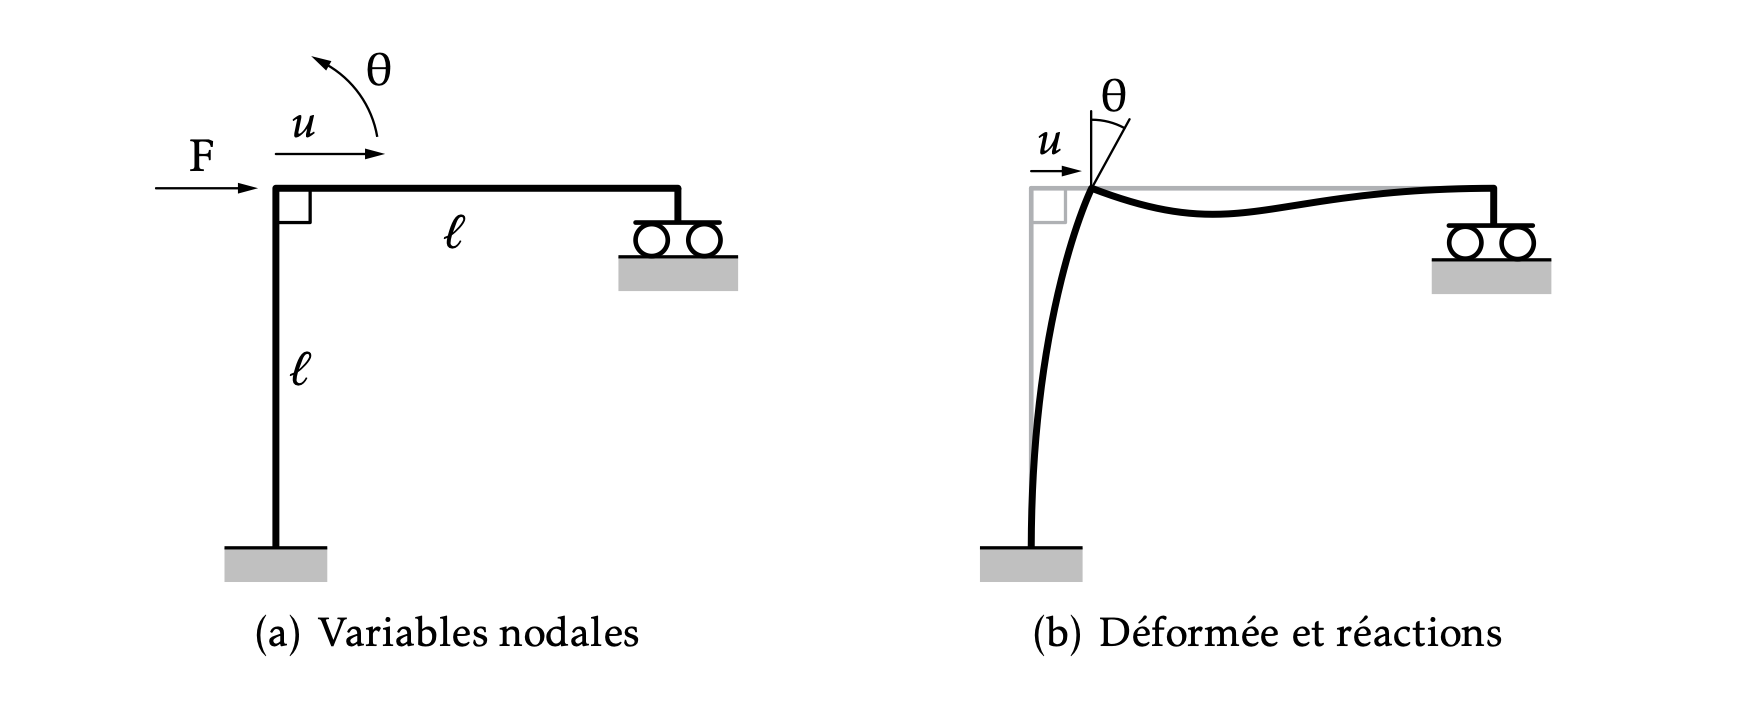
\includegraphics[scale=0.3]{portique.png}
 \end{center}
 
 
% \begin{center}
% \begin{tikzpicture}[scale=2]
%	\coordinate(A) at (0,0);
%	\coordinate(B) at (0,3);
%	\coordinate(C) at (3,3);
%	
%	\draw[ultra thick,anchor=south west,blue]
%		(A) node[anchor= south west]{A}
%		--(B) node[anchor=north]{B} 
%		--(C) node[anchor=south east]{C};
%		
%	%\pic at (A) {encastrg};
%	\draw[very thick,red,latex-] (B) --++(-1,0) node[anchor=east]{$F$};	
%	\pic at (3,3) {ponctuelle};
%	\draw[ultra thick,gray](-0.3,0)--(0.3,0);	
%\end{tikzpicture}
%\end{center}
 
 On trouve 
 \[u_B^x=\frac{2FL^3}{15EI},\qquad u_B^y=0,\qquad \theta_B=-\frac{FL^2}{10EI}\]
 
\subsection*{Représentation graphique d'une poutre déformée }
On représente graphiquement une poutre $AB$ par une courbe paramétrée polynomiale d'ordre 3 par l'application $P:[0,\ell]\to \mathbb{R}^2$ définie par 
\[P(s)=\left(1-\frac s{\ell}\right)^3A+3\left(1-\frac s{\ell}\right)^2\left(\frac s{\ell}\right)A_1+3\left(1-\frac s{\ell}\right)\left(\frac s{\ell}\right)^2B_1+\left(\frac s{\ell}\right)^3B\]
On a bien $P(0)=A$ et $P(\ell)=B$. On détermine $A_1$ et $B_1$ en supposant que $P'(s)$ est tangente à la déformée de la poutre en $s=0$ et $s=\ell$. On a $P'(0)=-\frac 3{\ell}\left(A-A_1\right)$ et $P'(\ell)=\frac 3{\ell}\left(B-B_1\right)$. D'où
\[ A_1=A+\frac{\ell}{3}P'(0),  \qquad B_1=B-\frac{\ell}{3}P'(\ell)\]
où
\[P'(s)=\frac{\de P}{\de s}=\left(\begin{array}{c}
\cos\varphi \\ \sin\varphi
\end{array}\right)=\left(\begin{array}{c}
\cos(\theta_0+\theta) \\ \sin(\theta_0+\theta)
\end{array}\right)=\left(\begin{array}{c}
\cos\theta_0\cos\theta-\sin\theta_0\sin\theta \\ \sin\theta_0\cos\theta+\cos\theta_0\sin\theta
\end{array}\right)\simeq \left(\begin{array}{c}
\cos\theta_0-\sin\theta_0\cdot\theta \\ \sin\theta_0+\cos\theta_0\cdot\theta
\end{array}\right)\]
où $\varphi$ est l'angle de la tangente avec $Ox$ qui n'est autre que l'angle que fait la poutre avec $Ox$ plus l'angle de flexion: $\varphi=\theta_0+\theta$. avec $\theta $ assez petit.


 \end{document}
 






